\chapter{Discrete Random Variables}

\section{Random Variables}

\begin{definition}
    A \vocab{random variable} is a variable whose possible values are numerical outcomes of a random experiment.
\end{definition}

Random variables are typically denoted by capital letters such as $X$ or $Y$.

There are two types of random variables: discrete and continuous.

\begin{definition}
    A \vocab{discrete random variable} is a random variable that assumes countable values $x_1$, $x_2$, $\dots$, $x_n$ (can be infinite).
\end{definition}

Examples of discrete random variables include the number that shows on the toss of a fair die ($X = 1, 2, \dots, 6$), and the number of times a fair die is thrown until a `6' is obtained ($Y = 1, 2, \dots,$ to infinity).

\begin{definition}
    A \vocab{continuous random variable} is a random variable that can take on any value in a given interval.
\end{definition}

Note that the value of a continuous random variable is uncountable. It can only take on an interval of values, not a specific value.

An example of continuous random variables is the volume of beverage (in ml) in a 500 ml bottle ($100 \leq X \leq 200$, $200 \leq X \leq 300$, etc.)

In this chapter, we will only discuss discrete random variables. We will deal more with continuous random variables in \SS\ref{chap:Continuous-Random-Variables}.

\section{Properties}

\subsection{Probability Distribution}

Since the values of a random variable are determined by chance, there is a distribution associated with them. We call this a probability distribution.

\begin{definition}
    A \vocab{probability distribution} describes all possible values of the random variable and their corresponding probabilities. It assigns a probability value to each possible outcome in the sample space.
\end{definition}

A probability distribution of a discrete random variable can be given in the form of a table, a graph or a mathematical formula.

Note that the particular values of a random variable are denoted by lower-case letters. For instance, the particular values of a random variable $X$ are denoted by $x$.

\begin{example}
    A single fair 6-sided die is thrown. Let $X$ be the random variable representing the number of dots showing on the die. Note that the possible values of $X$ are $x = 1, 2, 3, 4, 5, 6$.

    The probability distribution associated with $X$ can be given in table form:
    \begin{center}
        \begin{tabular}{|r|c|c|c|c|c|c|}
            \hline
            $x$ & 1 & 2 & 3 & 4 & 5 & 6 \\ \hline
            $\P{X = x}$ & $\frac16$ & $\frac16$ & $\frac16$ & $\frac16$ & $\frac16$ & $\frac16$ \\ \hline
        \end{tabular}
    \end{center}
    or expressed as a formula: \[\P{X = x} = \frac16, \quad x \in \bc{1, 2, 3, 4, 5, 6},\] or expressed as a graph:
    \begin{center}\tikzsetnextfilename{415}
        \begin{tikzpicture}
            \draw[->] (0, -1) -- (0, 2) node[anchor=east] {$\P{X = x}$};
            \draw[->] (-1, 0) -- (7, 0) node[anchor=west] {$x$};
            \draw (0.1, 1) -- (-0.1, 1) node[anchor=east] {$\frac16$};

            \draw (1, 1) -- (1, 0) node[anchor=north] {1};
            \draw (2, 1) -- (2, 0) node[anchor=north] {2};
            \draw (3, 1) -- (3, 0) node[anchor=north] {3};
            \draw (4, 1) -- (4, 0) node[anchor=north] {4};
            \draw (5, 1) -- (5, 0) node[anchor=north] {5};
            \draw (6, 1) -- (6, 0) node[anchor=north] {6};
        \end{tikzpicture}
    \end{center}
\end{example}

From the above example, the discrete random variable $X$ takes on only countable values, and that if we sum all probabilities, we get a total of 1. In fact, these are conditions that all discrete random variables must satisfy.

\begin{condition}[Discrete Random Variable]
    For $X$ to be a discrete random variable,
    \begin{itemize}
        \item $X$ can take only countable values (finite or infinitely many), and
        \item $X$ has a probability distribution such that $0 \leq \P{X = x} \leq 1$ for all $x$ and \[\sum_{x} \P{X = x} = 1.\]
    \end{itemize}
\end{condition}

\subsection{Expectation}

Recall that in descriptive statistics, the mean of a sample can be calculated as \[\text{Mean} = \frac{\sum xf}{n},\] where $x$ is a data value and $f$ is its frequency. In the case of a discrete random variable $X$, we can think of $x$ as a particular value of $X$, and $f/n$ as the probability that $x$ occurs (i.e. how ``frequently'' $x$ occurs). Thus, \[\text{Mean} = \sum_{x} x \P{X = x}.\] We call this ``mean'' the expectation of $X$.

\begin{definition}
    The \vocab{expectation}, or \vocab{expected value}, of $X$, denoted as $\E{X}$ or $\m$, is given by \[\E{X} = \sum_{x} x \P{X = x}.\]
\end{definition}

\begin{example}
    A single fair 6-sided die is thrown. Let $X$ be the random variable representing the number of dots showing on the die. Note that the possible values of $X$ are $x = 1, 2, 3, 4, 5, 6$. Since $\P{X = x} = \frac16$ for all possible values of $x$, the expectation of $X$ is given by \[\E{X} = \sum_{x = 1}^6 x\P{X = x} = \frac16 \sum_{x= 1}^6 x = 3.5.\]
\end{example}

Note that the phrase ``expected value of $X$'' refers to the long-term weighted average value of a random variable $X$ and is not a typical value that $X$ can take. In fact, a random variable might never be equal to its ``expected value''. For instance, in the above example, a 6-sided dice will clearly never roll a value of $3.5$.

We can generalize the notion of expectation to other functions involving $X$.

\begin{definition}
    Let $f(X)$ be any function of the discrete random variable $X$. Then \[\E{f(X)} = \sum_{x} f(x) \P{X = x}.\]
\end{definition}

For instance, $\E{10 X} = \sum 10 x \P{X = x}$, and $\E{X^2 - 4} = \sum (x^2 - 4) \P{X = x}$.

From the definition of $\E{f(X)}$, one can easily prove the following results:
\begin{proposition}[Properties of Expectation]
    For a real constant $a$,
    \begin{itemize}
        \item $\E{a} = a$,
        \item $\E{aX} = a\E{x}$,
        \item $\E{f_1(X) + f_2(X)} = \E{f_1(X)} + \E{f_2(X)}$, where $f_1$ and $f_2$ are functions of $X$.
    \end{itemize}
\end{proposition}

In fact, the last property is a direct consequence of the linearity of the expectation with respect to multiple random variables:

\begin{proposition}[Linearity of Expectation]
    Let $X$ and $Y$ be random variables (dependent or independent), and let $a$ and $b$ be real constants. Then \[\E{aX \pm bY} = a\E{X} \pm b\E{Y}.\]
\end{proposition}

\subsection{Variance}

Recall that in descriptive statistics, the variance of a sample can be calculated as \[\text{Variance} = \frac1n \sum f\bp{x - \bar x}^2,\] where $f$ is the frequency of a data value $x$ and $\bar x$ is the mean of the sample. In the context of discrete random variables, $\P{X = x}$ corresponds to $f/n$, while $\m$ corresponds to $\bar x$. Thus, \[\text{Variance} = \sum \bp{x - \m}^2 \P{X = x} = \E{(x- \m)^2}.\]

\begin{definition}
    The \vocab{variance} of a random variable $X$, denoted by $\Var{X}$ or $\s^2$, is defined as the expectation of the squared deviation of $X$ from the mean $\m$. Mathematically, \[\Var{X} = \E{\bp{X - \m}^2}.\]
\end{definition}

As motivated above, we can rewrite $\Var{X}$ solely in terms of expectations:

\begin{proposition}
    \[\Var{X} = \E{X^2} - \E{X}^2.\]
\end{proposition}
\begin{proof}
    \begin{align*}
        \Var{X} &= \E{\bp{X - \m}^2}\\
        &= \E{X^2 - 2\m X + \m^2}\\
        &= \E{X^2} - 2\m \E{X} + \m^2\\
        &= \E{X^2} - 2\E{X}^2 + \E{X}^2\\
        &= \E{X^2} - \E{X}^2.
    \end{align*}
\end{proof}

Compare this with the alternative expression for the variance used in descriptive statistics: \[\text{Variance} = \frac1n \sum fx^2 - \bp{\frac1n \sum fx}^2.\]

A small value for the variance indicates that most of the values that $X$ can take are clustered about the mean. Conversely, a higher value for the variance indicates that the values that $X$ can take are spread over a larger range about the mean.

Correspondingly, the \vocab{standard deviation}, which is the positive square root of the variance, is denoted by $\s$, i.e. \[\s = \sqrt{\Var{X}}.\]

From the definition of variance, one can easily prove the following properties:
\begin{proposition}[Properties of Variance]
    Given that $a$ and $b$ are real constants,
    \begin{itemize}
        \item $\Var{a} = 0$,
        \item $\Var{aX} = a^2 \Var{X}$,
        \item $\Var{aX + b} = a^2 \Var{X}$.
    \end{itemize}
\end{proposition}
\begin{proof}
    It suffices to prove the last statement. Applying the formula $\Var{X} = \E{X^2} - \E{X}^2$, we have
    \begin{align*}
        \Var{aX + b} &= \E{(aX + b)^2} - \E{aX + b}^2\\
        &= \E{a^2 X^2 + 2ab X + b^2} - \bp{a\E{X} + b}^2\\
        &= a^2\E{X^2} + 2ab \E{X} + b^2 - a^2 \E{X}^2 - 2ab \E{X} - b^2\\
        &= a^2 \bs{\E{X^2} -\E{X}^2}\\
        &= a^2 \Var{X}.
    \end{align*}
\end{proof}

Another important property is the variance of more than one random variable. In fact, the property $\Var{aX + b} = a^2 \Var{X}$ is a direct consequence of the statement below:

\begin{proposition}[Variance of More Than One Random Variable]
    If $X$ and $Y$ are two \emph{independent} variables, then \[\Var{aX \pm bY} = a^2 \Var{X} + b^2 \Var{Y}.\]
\end{proposition}

Notice that the sign on the RHS is always a `+' regardless of the sign on the LHS. Intuitively, we expect deviations to increase when combining more observations together, not reduce it.

\section{Binomial Distribution}

Consider an experiment which has two possible outcomes, one we term ``success'' and the other ``failure''. A binomial situation arises when $n$ independent trials of such experiments are performed.

Examples of such experiments are:
\begin{itemize}
    \item Tossing a fair coin 6 times (consider obtaining a head on a single toss as ``success'' and obtaining a tail as ``failure'').
    \item Shooting a target 5 times (consider hitting the bull's eye in each shot as ``success'' and not hitting the bull's eye as ``failure'').
\end{itemize}

\begin{condition}[Binomial Model]
    The conditions for a binomial model are:
    \begin{itemize}
        \item a finite number, $n$, trials are carried out,
        \item the trials are independent,
        \item the outcome of each trial is either a ``success'' or a ``failure'', and
        \item the probability of success, $p$, is the same for each trial.
    \end{itemize}
\end{condition}

\begin{definition}
    Let the random variable $X$ be the number of trials, out of $n$ trials, that are successful. If the above conditions are met, then $X$ is said to follow a \vocab{binomial distribution} with $n$ number of trials and probability of success $p$, written as \[X \sim \Binom{n}{p}.\]
\end{definition}

\begin{example}
    Recall the example of tossing a fair coin 6 times. This experiment clearly fits a binomial model:
    \begin{itemize}
        \item There are 6 tosses -- i.e. a finite number of trials.
        \item Given that the tosses likely take place one after another, the outcome of one toss will not affect the outcome of another toss -- i.e. the trials are independent.
        \item Each toss only results in a head or tail -- i.e. only two possible outcomes, a ``success'' or ``failure''.
        \item The probability of obtaining heads remains the same at $0.5$ for each toss -- i.e. the probability of success remains unchanged.
    \end{itemize}
\end{example}

\subsection{Probability Distribution}

\begin{proposition}[Probability Distribution of Binomial Distribution]
    Let the random variable $X \sim \Binom{n}{p}$. Then \[\P{X = x} = \binom{n}{x} p^x \bp{1 - p}^{n-x}.\]
\end{proposition}
\begin{proof}
    The event $X = x$ represents obtaining $x$ successes (and $n-x$ failures) out of $n$ total trials. The probability of $x$ successes is simply $p^x$, while the probability of $n-x$ failures is $(1-p)^{n-x}$. Since there are $\comb{n}{x}$ ways to choose the $x$ successes from $n$ total trials, the probability of having exactly $x$ successes, i.e. $\P{X = x}$, is \[\P{X = x} = \binom{n}{x} p^x \bp{1 - p}^{n-x}.\]
\end{proof}

\subsection{Expectation and Variance}

\begin{proposition}[Expectation of Binomial Distribution]
    For $X \sim \Binom{n}{p}$, \[\E{X} = np.\]
\end{proposition}
\begin{proof}
    Since probabilities sum to 1, we have \[\sum_{r = 0}^n \P{X = r} = \sum_{r = 0}^n \binom{n}{r} p^r (1-p)^{n-r} = 1.\] Differentiating this with respect to $p$, we have \[\sum_{r = 0}^n \binom{n}{r} \bs{r p^{r-1} (1-p)^{n-r} - (n-r) p^r (1-p)^{n-r-1}} = 0.\] We can expand the LHS as \[\frac1p \sum_{r = 0}^n r \binom{n}{r} p^{r} (1-p)^r - \frac{n}{1-p} \sum_{r = 0}^n \binom{n}{r} p^r (1-p)^{n-r} + \frac{1}{1-p} \sum_{r = 0}^n r \binom{n}{r} p^r (1-p)^{n-r} = 0.\] Rewriting this in terms of $\P{X = r}$ yields \[\frac1p \underbrace{\sum_{r = 0}^n r \P{X = r}}_{\E{X}} - \frac{n}{1-p} \underbrace{\sum_{r =0}^n \P{X = r}}_{1} + \frac1{1-p} \underbrace{\sum_{r = 0}^n r \P{X = r}}_{\E{X}} = 0.\] Thus, \[\frac1p \E{X} - \frac{n}{1-p} + \frac1{1-p} \E{X} = 0 \implies \E{X} = np.\]
\end{proof}

\begin{proposition}[Variance of Binomial Distribution]
    For $X \sim \Binom{n}{p}$, \[\Var{X} = np(1-p).\]
\end{proposition}
\begin{proof}
    One can use a similar trick (differentiating $\E{X} = np$) to obtain \[\E{X^2} = np(1 - p + np).\] Thus, \[\Var{X} = \E{X^2} - \E{X}^2 = np(1 - p + np) - (np)^2 = np(1-p).\]
\end{proof}

\subsection{Graphs of Probability Distribution}

Given that $X \sim \Binom{n}{p}$, the graphs of the probability distribution of $X$ for various values of $n$ and $p$ are shown below.

\begin{minipage}{0.49\textwidth}
    \centering
    \tikzsetnextfilename{37}
    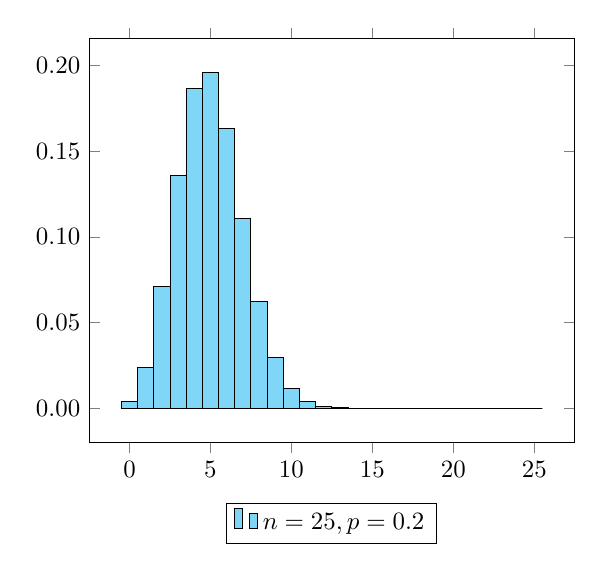
\begin{tikzpicture}[
        scale=0.9,
        declare function={binom(\k,\n,\p)=\n!/(\k!*(\n-\k)!)*\p^\k*(1-\p)^(\n-\k);}
    ]
    \begin{axis}[
        samples at={0,...,25},
        yticklabel style={
            /pgf/number format/fixed,
            /pgf/number format/fixed zerofill,
            /pgf/number format/precision=2
        },
        legend style={at={(0.5, -0.15)},anchor=north},
        ybar=0pt, bar width=1
    ]
    \addplot [fill=cyan, fill opacity=0.5] {binom(x,25,0.2)}; \addlegendentry{$n=25,p=0.2$}
    \end{axis}
    \end{tikzpicture}
\end{minipage}
\begin{minipage}{0.49\textwidth}
    \centering
    \tikzsetnextfilename{44}
    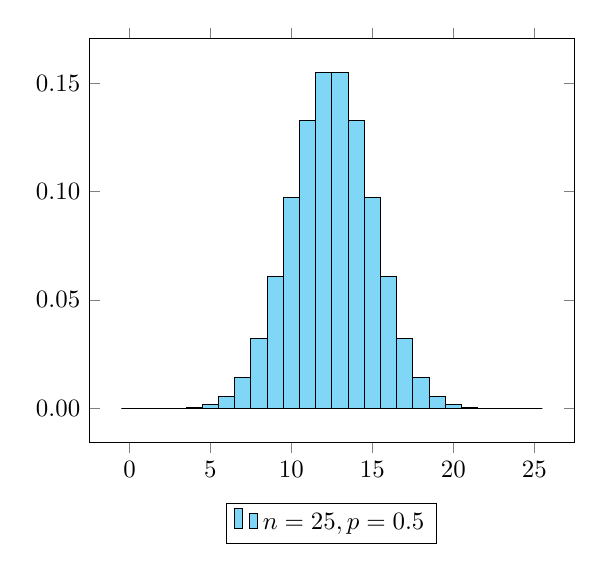
\begin{tikzpicture}[
        scale=0.9,
        declare function={binom(\k,\n,\p)=\n!/(\k!*(\n-\k)!)*\p^\k*(1-\p)^(\n-\k);}
    ]
    \begin{axis}[
        samples at={0,...,25},
        yticklabel style={
            /pgf/number format/fixed,
            /pgf/number format/fixed zerofill,
            /pgf/number format/precision=2
        },
        legend style={at={(0.5, -0.15)},anchor=north},
        ybar=0pt, bar width=1
    ]
    \addplot [fill=cyan, fill opacity=0.5] {binom(x,25,0.5)}; \addlegendentry{$n=25,p=0.5$}
    \end{axis}
    \end{tikzpicture}
\end{minipage}

\begin{center}
    \tikzsetnextfilename{416}
    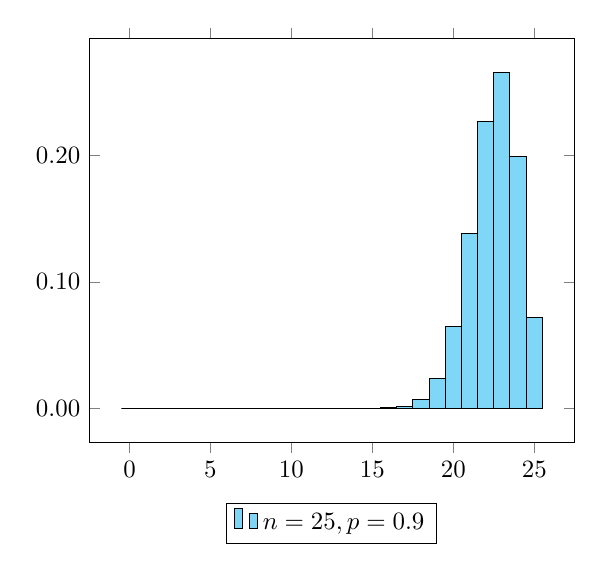
\begin{tikzpicture}[
        scale=0.9,
        declare function={binom(\k,\n,\p)=\n!/(\k!*(\n-\k)!)*\p^\k*(1-\p)^(\n-\k);}
    ]
    \begin{axis}[
        samples at={0,...,25},
        yticklabel style={
            /pgf/number format/fixed,
            /pgf/number format/fixed zerofill,
            /pgf/number format/precision=2
        },
        legend style={at={(0.5, -0.15)},anchor=north},
        ybar=0pt, bar width=1
    ]
    \addplot [fill=cyan, fill opacity=0.5] {binom(x,25,0.9)}; \addlegendentry{$n=25,p=0.9$}
    \end{axis}
    \end{tikzpicture}
\end{center}

Notice that
\begin{itemize}
    \item when $p$ is low, the graph is skewed to the left, i.e. probabilities are larger for lower values of $X$,
    \item when $p$ is high, the graph is skewed to the right, i.e. probabilities are larger for higher values of $X$, and
    \item when $p = 0.5$, we get a symmetrical distribution.
\end{itemize}

Also note that a binomial distribution can only have 1 or 2 modes. In addition, if there are 2 modes, they must be adjacent to each other, i.e. they differ by 1.

\section{Poisson Distribution}

\begin{definition}
    Let $X$ be the number of occurrences of a particular event over an interval of time (or space) $t$. Let $\l$ be the mean rate of occurrence per unit time. Then $X$ is said to follow a Poisson distribution with parameter $\l t$, written as \[X \sim \Po{\l t}.\]
\end{definition}
\begin{remark}
    Typically, we assume $t$ to be the unit time interval, in which case we simply write $X \sim \Po{\l}$.
\end{remark}

For $X$ to follow the Poisson distribution, the following conditions must also be fulfilled:

\begin{condition}[Poisson Model]\label{con:Poisson}
    \phantom{.}
    \begin{itemize}
        \item Events must be independent.
        \item Events occur singly (i.e. the chances of 2 or more occurrences at precisely the same point in time (or space) is negligible) and randomly.
        \item Events occur at a constant average rate, i.e. for a given interval of time (or space), the mean number of occurrences is proportional to the length of the interval.
    \end{itemize}
\end{condition}

Situations where a Poisson model could be used include:
\begin{itemize}
    \item the number of car accidents on a stretch of road on a random day, and
    \item the number of raisins per 10 cm$^3$ of a chocolate bar.
\end{itemize}

\subsection{Probability Distribution}

\begin{proposition}[Probability Distribution of Poisson Distribution]
    Let $X \sim \Po{\l t}$. Then \[\P{X = x} = \e^{-\l t} \frac{(\l t)^x}{x!}, \quad x \in \NN_{0}.\]
\end{proposition}
We will present two proofs/derivations for the probability distribution of the Poisson distribution. The first proof (adapted from a \href{https://www.pp.rhul.ac.uk/~cowan/stat/notes/PoissonNote.pdf}{note} by Cowan) involves infinitesimals and differential equations, while the second proof (adapted from a \href{https://blog.kalculate.ai/2024/03/27/poisson-distribution/}{blog post}) uses a measure-theoretic argument.
\begin{proof}[Proof 1 (Differential Equations).]
    Suppose $X$ is the number of occurrences of an event over some time interval $t$. We can divide this interval into infinitely short subintervals $\D t$. For convenience, let $\P{x; t}$ be the probability that exactly $x$ events happen in the time interval $t$.

    Since $\l$ is the mean rate of occurrence, we have \[\P{1; \D t} = \l \D t.\] Additionally, since $\D t$ is infinitely short, we can assume that either one event occurs, or no event occurs, i.e. \[\P{0; \D t} = 1 - \P{1; \D t} = 1 - \l \D t.\]

    We now wish to find an expression for $\P{x;t}$. To do so, we first consider $\P{0;t}$. Suppose we extend the time interval $t$ by $\D t$. Since events occur independently and randomly, we must have \[\P{0;t + \D t} = \P{0; t} \P{0; \D t} = \P{0;t} \bp{1 - \l \D t}.\] We can rearrange this to get \[-\l \P{0;t} = \frac{\P{0;t + \D t} - \P{0;t}}{\D t} = \der{}{t} \P{0;t}.\] $\P{0;t}$ thus satisfies the differential equation \[\der{}{t} \P{0;t} = -\l \P{0;t},\] which has solution \[\P{0;t} = C \e^{-\l t}.\] Since no event can happen in a time interval of 0 seconds, we have \[\P{0;0} = 1 \implies C = 1.\] Thus, \[\P{0; t} = \e^{-\l t}. \tag{1}\]

    We now consider $\P{x;t + \D t}$, where $x \neq 0$. If $x$ events have occurred in a time interval of $t + \D t$, one of two things must have occurred:
    \begin{itemize}
        \item There were $x$ events in the first $t$ seconds, but none in the last $\D t$.
        \item There were $x-1$ events in the first $t$ seconds, and one in the last $\D t$.
    \end{itemize}
    We hence have
    \begin{align*}
        \P{x; t + \D t} &= \P{x;t}\P{0;\D t} + \P{x-1 ; t} \P{1; \D t}\\
        &= \P{x;t} (1 - \l \D t) + \P{x-1;t} \l \D t.
    \end{align*}
    Rearranging, we get a differential equation involving $\P{x;t}$: \[\der{}{t} \P{x;t} + \l \P{x;t} = \l \P{x-1;t}.\] Multiplying through by the integrating factor $\e^{\l t}$, we get \[\der{}{t} \bs{\e^{\l t }\P{x;t}} = \l \e^{\l t} \P{x-1;t}. \tag{2}\]
    
    We now induct on (2) to get an expression for $\P{x;t}$. We claim that \[\P{x;t} = \frac{(\l t)^x}{x!} \e^{-\l t}.\] We have already shown that this holds for the $x = 0$ case. Now, substituting $x + 1$ into (2), we get \[\der{}{t} \bs{\e^{\l t }\P{x+1;t}} = \l \e^{\l t} \P{x;t} = \l \e^{\l t} \bs{\frac{(\l t)^x}{x!} \e^{-\l t}} = \frac{\l^{x+1} t^x}{x!}.\] Integrating and simplifying, we get \[\P{x+1;t} = \e^{-\l t} \int \frac{\l^{x+1} t^x}{x!} \d t = \frac{(\l t)^{x+1}}{(x+1)!} \e^{-\l t} + C \e^{-\l t}.\] Since $\P{x+1;0} = 0$, we have $C = 0$, whence \[\P{x+1;t} = \frac{(\l t)^{x+1}}{(x+1)!} \e^{-\l t}.\] This closes the induction, and we conclude that \[\P{X = x} = \P{x;t} = \frac{(\l t)^x}{x!} \e^{-\l t}.\]
\end{proof}

\begin{proof}[Proof 2 (Measure Theory).]
    Suppose $x$ events occur in the time interval $[0, t)$, and let their times be given by the unordered $x$-tuple $(t_1, t_2, \dots, t_x)$. Without loss of generality, we take $0 \leq t_1 < t_2 < \dots < t_x < t$. Let $S_x$ be the set of all such $x$-tuples. Since $\l$ is the mean rate of events per unit time, we define the measure $\m$ such that $\m([0, 1)) = \l$.

    Consider the set $T = [0, t)^x$ of all ordered $x$-tuples. Its measure is given by \[\m(T) = \m([0, t)^x) = (t \m([0, 1))^x = (\l t)^x.\] Define the equivalence relation $\sim$ on $T$ such that any two $x$-tuples $u = (u_1, u_2, \dots, u_x)$ and $v = (v_1, v_2, \dots, v_x)$ in $T$, \[u \sim v \iff \bc{u_1, u_2, \dots, u_x} = \bc{v_1, v_2, \dots, v_x}.\] Then the quotient set $T / \sim$ is exactly $S$. Furthermore, since $\sim$ partitions $T$ into equivalence classes of size $x!$, it follows that \[\m(S) = \frac{\m(T)}{x!} = \frac{(\l t)^x}{x!}.\]
    
    Now consider the sample space $S$, which is given by \[S = \bigcup_{x = 0}^\infty S_x.\] Since all $S_x$ are disjoint, the measure of $S$ is simply \[\m(S) = \sum_{x = 0}^\infty \m(S_x) = \sum_{x = 0}^\infty \frac{(\l t)^x}{x!} = \e^{\l t}.\]

    Thus, the probability that exactly $x$ events occur in time $t$ is given by the ratio \[\frac{\m(S_x)}{\m(S)} = \frac{(\l t)^x / x!}{\e^{\l t}} = \e^{-\l t} \frac{(\l t)^x}{x!}.\]
\end{proof}

Let $X$ and $Y$ measure the number of events $E$ and $F$ over some time interval. Then $X + Y$ counts the event $G = X + Y$ over the same time interval. Intuitively, $X + Y$ should follow a Poisson distribution since it satisfies the three conditions (\ref{con:Poisson}):

\begin{itemize}
    \item $G$ is independent: Since $X$ and $Y$ both follow a Poisson distribution, $E$ and $F$ must both occur independently. Since $X$ and $Y$ are independent of each other, $E$ and $F$ are also independent of each other. Thus, $G$ occurs independently.
    \item $G$ occurs singly and randomly.
    \item $G$ occurs at a constant average rate: Since $E$ occurs with constant random rate $\l_1$, and $F$ occurs with constant random rate $\l_2$, we expect $G$ to also occur with constant random rate $\l_1 + \l_2$.
\end{itemize}

We can prove this statement more rigorously using the probability distribution of a Poisson random variable:

\begin{proposition}[Sum of Independent Poisson Random Variables is a Poisson Random Variable]
    Let $X \sim \Po{\l_1}$, $Y \sim \Po{\l_2}$ be independent random variables. Then $X + Y \sim \Po{\l_1 + \l_2}$
\end{proposition}
\begin{proof}
    Consider the event $X + Y = n$. This can only happen if $X = m$ and $Y = n - m$. Thus, \[\P{X + Y = n} = \sum_{m = 0}^n \P{X = m \land Y = n -m}.\] Since $X$ and $Y$ are independent, we can split the summands into products: \[\P{X + Y = n} = \sum_{m = 0}^n \P{X = m} \P{Y = n -m}.\] Using the probability distribution we derived earlier, \[\P{X + Y = n} = \sum_{m = 0}^n \bs{\e^{-\l_1} \frac{\l_1^m}{m!}} \bs{\e^{-\l_2} \frac{\l_2^{n-m}}{(n-m)!}} = \frac{\e^{-(\l_1 + \l_2)}}{n!} \sum_{m = 0}^n \frac{n!}{m! (n-m)!} \l_1^m \l_2^{n-m}.\] Observe that the sum is simply the binomial expansion of $(\l_1 + \l_2)^{n}$. Thus, \[\P{X + Y = n} = \e^{-(\l_1 + \l_2)} = \frac{(\l_1 + \l_2)^n}{n!},\] which is exactly the probability distribution of a Poisson random variable with parameter $\l_1 + \l_2$.
\end{proof}

\subsection{Expectation and Variance}


\begin{proposition}[Expectation of Poisson Distribution]
    Let $X \sim \Po{\l t}$. Then $\E{X} = \l t$.
\end{proposition}
Recall that we defined $\l$ as the mean rate of occurrence per unit time. Since we measure $X$ over a time interval of length $t$, the mean number of events, $\E{X}$, is simply $\l t$. We can verify this with the following calculation:
\begin{proof}
    \begin{gather*}
        \E{X} = \sum_{x = 0}^\infty  x \P{X = x} = \sum_{x = 1}^\infty  x \P{X = x} = \sum_{x = 1}^\infty  x \e^{-\l t} \frac{(\l t)^x}{x!}\\
        = \l t \e^{-\l t} \sum_{x = 1}^\infty \frac{(\l t)^{x-1}}{(x-1)!} = \l t \e^{-\l t} \sum_{x = 0}^\infty \frac{(\l t)^x}{x!} = \l t \e^{-\l t} \e^{\l t} = \l t.
    \end{gather*}
\end{proof}

\begin{proposition}[Variance of Poisson Distribution]
    Let $X \sim \Po{\l t}$. Then $\Var{X} = \l t$.
\end{proposition}
\begin{proof}[Proof 1.]
    Consider $\E{X^2 - X} = \E{X(X-1)}$.
    \begin{gather*}
        \E{X(X-1)} = \sum_{x = 0}^\infty x(x-1) \P{X = x} = \sum_{x = 2}^\infty x(x-1)\P{X = x}\\
        = (\l t)^2 \e^{-\l t} \sum_{x = 2}^\infty \frac{(\l t)^{x-2}}{(x-2)!} = (\l t)^2 \e^{-\l t} \e^{\l t} = (\l t)^2.
    \end{gather*}
    Thus, $\E{X^2} = \E{X^2 - X} + \E{X} = (\l t)^2 + \l t$, from which it follows \[\Var{X} = \E{X^2} - \E{X}^2 = \l t.\]
\end{proof}
\begin{proof}[Proof 2.]
    Partition the time interval on which we measure $X$ into $n$ equal subdivisions. Let $Y_i$ measure the number of events that occur in the $i$th subdivision. As $n \to \infty$, each $Y_i$ approaches a point, in which case $Y_i$ follows a Bernoulli distribution with probability of success $p = \E{Y_i} = \l t / n$. Thus, \[\Var{Y_i} = p(1-p) = \frac{\l t}n \bp{1 - \frac{\l t}n}.\] Since the events occur independently, the variance of $X$ is simply the sum of the variances of $Y_i$. We thus obtain \[\Var{X} = \lim_{n \to \infty} \sum_{i = 1}^n \Var{Y_i} = \lim_{n \to \infty} \sum_{i = 0}^n \frac{\l t}n \bp{1 - \frac{\l t}n} = \lim_{n \to \infty} n\bp{\frac{\l t}{n}}\bp{1 - \frac{\l t}{n}} = \l t.\]
\end{proof}

\subsection{Graphs of Probability Distributions}

Given that $X \sim \Po{\l}$, the graphs of the probability distribution of $X$ for various values of $\l$ are shown below:

\begin{minipage}{0.49\textwidth}
    \centering
    \tikzsetnextfilename{417}
    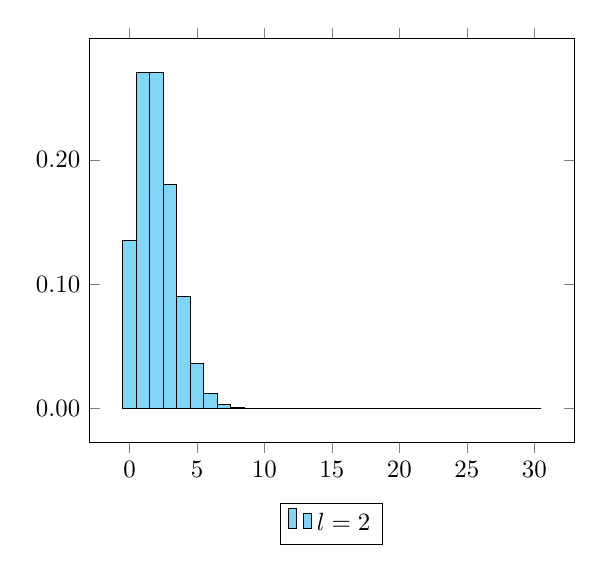
\begin{tikzpicture}[
        scale=0.9,
        declare function={poisson(\k,\l)=e^(-\l) * \l^(\k) / (\k)!;},
    ]
    \begin{axis}[
        samples at={0,...,30},
        yticklabel style={
            /pgf/number format/fixed,
            /pgf/number format/fixed zerofill,
            /pgf/number format/precision=2
        },
        legend style={at={(0.5, -0.15)},anchor=north},
        ybar=0pt, bar width=1
    ]
    \addplot [fill=cyan, fill opacity=0.5] {poisson(x,2)}; \addlegendentry{$\l=2$}
    \end{axis}
    \end{tikzpicture}
\end{minipage}
\begin{minipage}{0.49\textwidth}
    \centering
    \tikzsetnextfilename{418}
    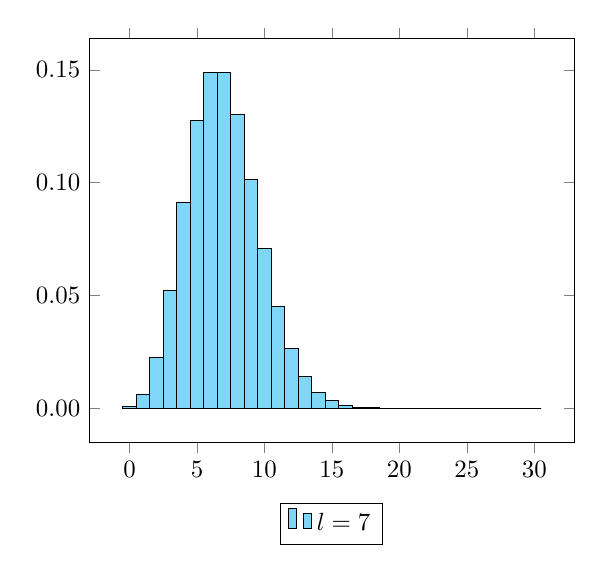
\begin{tikzpicture}[
        scale=0.9,
        declare function={poisson(\k,\l)=e^(-\l) * \l^(\k) / (\k)!;},
    ]
    \begin{axis}[
        samples at={0,...,30},
        yticklabel style={
            /pgf/number format/fixed,
            /pgf/number format/fixed zerofill,
            /pgf/number format/precision=2
        },
        legend style={at={(0.5, -0.15)},anchor=north},
        ybar=0pt, bar width=1
    ]
    \addplot [fill=cyan, fill opacity=0.5] {poisson(x,7)}; \addlegendentry{$\l=7$}
    \end{axis}
    \end{tikzpicture}
\end{minipage}

\begin{center}
    \tikzsetnextfilename{419}
    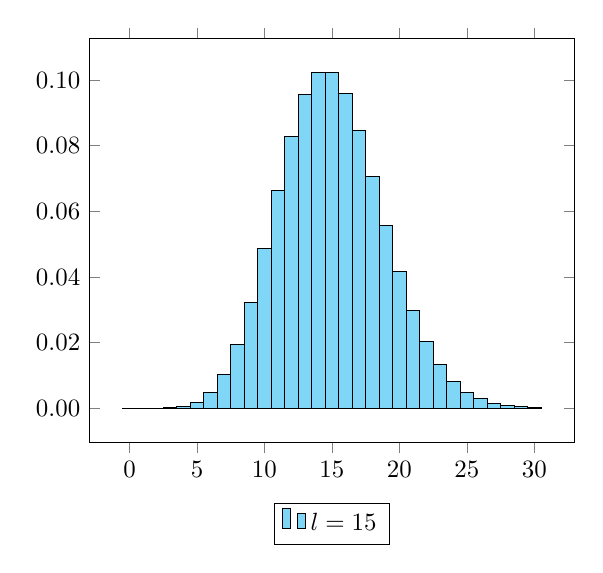
\begin{tikzpicture}[
        scale=0.9,
        declare function={poisson(\k,\l)=e^(-\l) * \l^(\k) / (\k)!;},
    ]
    \begin{axis}[
        samples at={0,...,30},
        yticklabel style={
            /pgf/number format/fixed,
            /pgf/number format/fixed zerofill,
            /pgf/number format/precision=2
        },
        legend style={at={(0.5, -0.15)},anchor=north},
        ybar=0pt, bar width=1
    ]
    \addplot [fill=cyan, fill opacity=0.5] {poisson(x,15)}; \addlegendentry{$\l=15$}
    \end{axis}
    \end{tikzpicture}
\end{center}

\subsection{Poisson Distribution as an Approximation to the Binomial Distribution}

\begin{proposition}
    If $X \sim \Binom{n}{p}$ and $n$ is large ($n > 50$) and $p$ is small ($p < 0.1$), then $X$ can be approximated by $\Po{\l}$, where $\l = np$.
\end{proposition}
\begin{proof}
    We know that \[\P{X = k} = \binom{n}{k} p^k (1 - p)^{n-k}. \tag{1}\] Since $n$ is large relative to $k$, we have \[\binom{n}{k} = \frac{n(n-1)(n-2)\dots(n-k+1)}{k!} \approx \frac{n^k}{k!}. \tag{2}\]
    
    Note also that \[(1-p)^{n-k} = \e^{(n-k) \ln{1-p}}.\] Since $p$ is small, we have $\ln{1-p} \approx -p$. Since $n$ is large relative to $k$, we have $n-k \approx n$. Thus, \[(1-p)^{n-k} \approx \e^{-pn}. \tag{3}\]

    Substituting (2), (3) and $\l = pn$ into (1), we get the approximation \[\P{X = k} \approx \frac{n^k}{k!} p^k \e^{-pn} = \e^{-\l} \frac{n^k}{k!} \bp{\frac{\l}{n}}^k = \e^{-\l} \frac{\l^k}{k!}.\]

    Thus, $X$ is approximately a Poisson distribution where $X \sim \Po{\l}$, where $\l = np$.
\end{proof}

The approximation gets better as $n$ gets larger and $p$ gets smaller, as the following diagrams illustrate.

\begin{minipage}{0.49\textwidth}
    \centering
    \tikzsetnextfilename{420}
    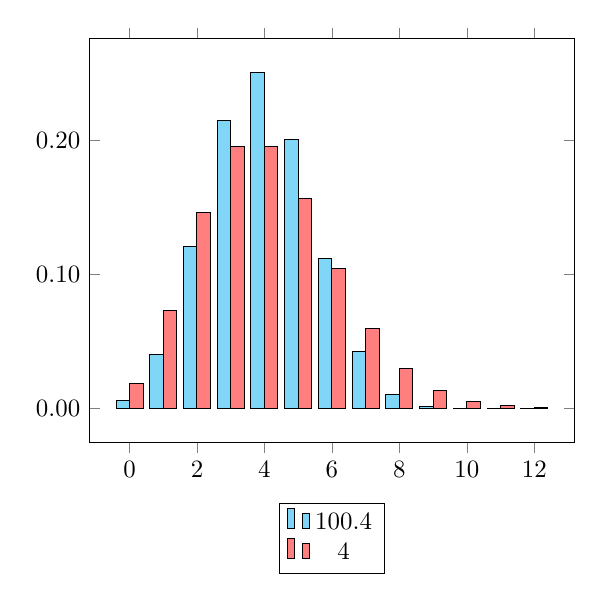
\begin{tikzpicture}[
        scale=0.9,
        declare function={poisson(\k,\l)=e^(-\l) * \l^(\k) / (\k)!;},
        declare function={binom(\k,\n,\p)=\n!/(\k!*(\n-\k)!)*\p^\k*(1-\p)^(\n-\k);}
    ]
    \begin{axis}[
        samples at={0,...,12},
        yticklabel style={
            /pgf/number format/fixed,
            /pgf/number format/fixed zerofill,
            /pgf/number format/precision=2
        },
        legend style={at={(0.5, -0.15)},anchor=north},
        ybar=0pt, bar width=0.4
    ]
    \addplot [fill=cyan, fill opacity=0.5] {binom(x,10,0.4)}; \addlegendentry{$\Binom{10}{0.4}$};
    \addplot [fill=red, fill opacity=0.5] {poisson(x,4)}; \addlegendentry{$\Po{4}$};
    \end{axis}
    \end{tikzpicture}
\end{minipage}
\begin{minipage}{0.49\textwidth}
    \centering
    \tikzsetnextfilename{422}
    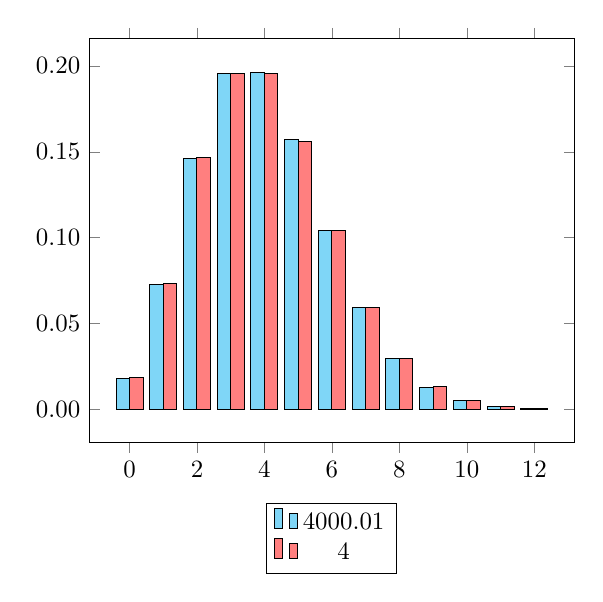
\begin{tikzpicture}[
        scale=0.9,
        declare function={poisson(\k,\l)=e^(-\l) * \l^(\k) / (\k)!;},
        declare function={binom(\k,\n,\p)=\n!/(\k!*(\n-\k)!)*\p^\k*(1-\p)^(\n-\k);}
    ]
    \begin{axis}[
        samples at={0,...,12},
        yticklabel style={
            /pgf/number format/fixed,
            /pgf/number format/fixed zerofill,
            /pgf/number format/precision=2
        },
        legend style={at={(0.5, -0.15)},anchor=north},
        ybar=0pt, bar width=0.4
    ]
    \addplot [fill=cyan, fill opacity=0.5] {binom(x,400,0.01)}; \addlegendentry{$\Binom{400}{0.01}$};
    \addplot [fill=red, fill opacity=0.5] {poisson(x,4)}; \addlegendentry{$\Po{4}$};
    \end{axis}
    \end{tikzpicture}
\end{minipage}

\medskip

This relationship between the binomial and Poisson distributions is particularly useful when we wish to find the sum of two binomial distributions. Consider two random variables $X_1 \sim \Binom{n_1}{p_1}$ and $X_2 \sim \Binom{n_2}{p_2}$, and let $Y = X_1 + X_2$. If we stick with binomial distributions, finding $\P{Y = k}$ would be a nightmare, as we would have to enumerate through all possible cases and calculate many terms: \[\P{Y = k} = \sum_{i = 0}^k \P{X_1 = i}\P{X_2 = k - i}.\] However, if we use approximate $X_1$ and $X_2$ using the Poisson distribution, i.e. $X_1 \sim \Po{\l_1}$ and $X_2 \sim \Po{\l_2}$, we immediately have $Y \sim \Po{\l_1 + \l_2}$, and we can easily approximate $\P{Y = k}$: \[\P{Y = k} \approx \e^{-(\l_1 + \l_2)} \frac{(\l_1 + \l_2)^k}{k!}.\]

\section{Geometric Distribution}

\begin{definition}
    Let $X$ be the number of trials up to and including the first success. Then $X$ follows a \vocab{geometric distribution} with probability of success $p$, denoted $X \sim \Geo{p}$.
\end{definition}

\begin{condition}[Conditions for Geometric Distribution]
    The conditions for a geometric model are:
    \begin{itemize}
        \item The trials are independent.
        \item There are only two possible outcomes to each trial, which we will call ``success'' and ``failure''.
        \item The probability of ``success'', $p$, is the same for each trial.
    \end{itemize}
\end{condition}

Note that the geometric model requires the same conditions as the binomial model, with the exception that the number of trials need not be finite. Intuitively, one could be extremely unlucky and keep on failing.

Situations where the geometric model could be applied to include:
\begin{itemize}
    \item The number of cards drawn from a pack (with replacement) before an ace is drawn.
    \item The number of times a fisherman casts a line into a river before he catches a fish.
\end{itemize}

\subsection{Probability Distribution}

\begin{proposition}[Probability Distribution of Geometric Distribution]
    Let $X \sim \Geo{p}$. Then \[\P{X = x} = (1-p)^{x-1} p, \quad x \in \ZZ^+.\]
\end{proposition}
\begin{proof}
    By definition, the event $X = x$ can only occur if the previous $x - 1$ trials are failures (which occur with probability $1-p$), and the $x$th trial is a success (which occur with probability $p$). Thus, \[\P{X = x} = \bp{1 - p}^{x-1} p.\]
\end{proof}

The geometric distribution has the following useful property:
\begin{proposition}
    Let $X \sim \Geo{p}$. Then \[\P{X > x} = (1-p)^x.\]
\end{proposition}
\begin{proof}[Proof 1.]
    The event $X > x$ is equivalent to the event that the first $x$ trials were all failures. Thus, $\P{X = x} = (1-p)^x$.
\end{proof}
\begin{proof}[Proof 2 (Probability Distribution).]
    We have \[\P{X > x} = \sum_{k = x + 1}^\infty \P{X = k} = \sum_{k = x+1}^\infty (1-p)^{k-1} p.\] This is simply an infinite geometric series with common ratio $1-p$ and first term $(1-p)^x p$. Thus, \[\P{X > x} = \frac{(1-p)^x p}{1 - (1-p)} = (1-p)^x.\]
\end{proof}

This actually implies a much stronger property about the geometric distribution:

\begin{definition}
    A random variable $X$ is said to be \vocab{memoryless} if \[\P{X > s + t}{X > t} = \P{X > s}\] for all non-negative $s$, $t$.
\end{definition}

\begin{proposition}[Geometric Distribution is Memoryless]
    Let $X \sim \Geo{p}$. Then $X$ is memoryless.
\end{proposition}
\begin{proof}
    \begin{gather*}
        \P{X > s + t}{X > t} = \frac{\P{X > s + t \and X > t}}{\P{X > t}} = \frac{\P{X > s + t}}{\P{X > t}}\\
        = \frac{(1-p)^{s+t}}{(1-p)^t} = (1-p)^s = \P{X > s}.
    \end{gather*}
\end{proof}

Intuitively, this means that having $s$ more observations before a success does not depend on there already being $t$ observations of failure. In other words, the ``waiting time'' for a success does not depend on how much ``time'' has already passed.

\subsection{Expectation and Variance}

\begin{proposition}[Expectation of Geometric Distribution]
    Let $X \sim \Geo{p}$. Then \[\E{X} = \frac1p.\]
\end{proposition}
\begin{proof}[Proof 1.]
    Intuitively, since each trial has probability of success $p$, we expect $p$ successes for every 1 trial. This is equivalent to 1 success every $1/p$ trials. Hence, $\E{X} = 1/p$.
\end{proof}
Of course, we can prove this fact more rigorously:
\begin{proof}[Proof 2 (Probability Distribution).]
    \[\E{X} = \sum_{k = 1}^\infty k \P{X = k} = p \sum_{k = 1}^\infty k (1-p)^{k-1}.\] Recall that the Maclaurin series of $(1 - x)^{-2}$ is \[\frac1{(1-x)^{2}} = \sum_{k = 1}^\infty k x^{k-1}.\] Substituting $1-p$ for $x$, we get \[\E{X} = \frac{p}{p^2} = \frac{1}{p}.\]
\end{proof}
\begin{proof}[Proof 3 (Memoryless Property).]
    The first trial can result in one of two outcomes:
    \begin{itemize}
        \item The first trial is a success (occurs with probability $p$). If this happens, the process stops, and $X = 1$.
        \item The first trial is a failure (occurs with probability $1-p$). If this happens, the process effectively ``restarts'' (memoryless property). The expected number of trials in this case becomes $\E{1 + X} = 1 + \E{X}$.
    \end{itemize}

    The expectation of $X$ can thus be calculated as:
    \begin{align*}
        \E{X} &= \P{\text{success}} \bp{\text{\# trials if success}} + \P{\text{failure}} \bp{\text{\# trials if failure}}\\
        &= (p)(1) + (1-p)\E{1 + X}
    \end{align*}
    Simplifying, we have $\E{X} = 1/p$.
\end{proof}

\begin{proposition}[Variance of Geometric Distribution]
    Let $X \sim \Geo{p}$. Then \[\Var{X} = \frac{1-p}{p^2}.\]
\end{proposition}
\begin{proof}[Proof 1 (Probability Distribution).]
    Recall that \[\sum_{k = 1}^\infty x^k = \frac{1}{1 - x}.\] Differentiating this twice with respect to $x$, we get \[\sum_{k = 1}^\infty k(k-1) x^{k-2} = \frac{2}{(1-x)^3} \implies \sum_{k = 1}^\infty \bp{k^2 - k} x^{k-1} = \frac{2x}{(1-x)^3}. \tag{1}\]

    Now consider $\E{X^2} - \E{X}$: \[\E{X^2} - \E{X}= \sum_{k = 1}^\infty \bp{k^2 - k} \P{X = k} = p \sum_{k = 1}^\infty \bp{k^2 - k} (1-p)^{k-1}.\] Using (1) with $x = 1-p$, \[\E{X^2} - \E{X} = p \bs{\frac{2(1-p)}{p^3}} = \frac{2 - 2p}{p^2}.\] Thus, \[\E{X^2} = \frac{2 - 2p}{p^2} + \frac1p = \frac{2-p}{p^2} \implies \Var{X} = \E{X^2} - \E{X}^2 = \frac{1-p}{p^2}.\]
\end{proof}
\begin{proof}[Proof 2 (Memoryless Property).]
    Following the memoryless property proof above, we have 
    \begin{align*}
        \E{X^2} &= \P{\text{success}} \bp{\text{\# trials if success}}^2 + \P{\text{failure}} \bp{\text{\# trials if failure}}^2\\
        &= (p)(1)^2 + (1-p)\E{(1 + X)^2}\\
        &= p + (1-p)\bs{1 + \frac2p + \E{X^2}}
    \end{align*}
    Simplifying, we have \[\E{X^2} = \frac{2-p}{p^2} \implies \Var{X} = \E{X^2} - \E{X}^2 = \frac{1-p}{p^2}.\]
\end{proof}

\subsection{Graphs of Probability Distribution}

Given that $X \sim \Geo{p}$, the graphs of the probability distribution of $X$ for various values of $p$ are shown below:

\begin{minipage}{0.49\textwidth}
    \centering
    \tikzsetnextfilename{423}
    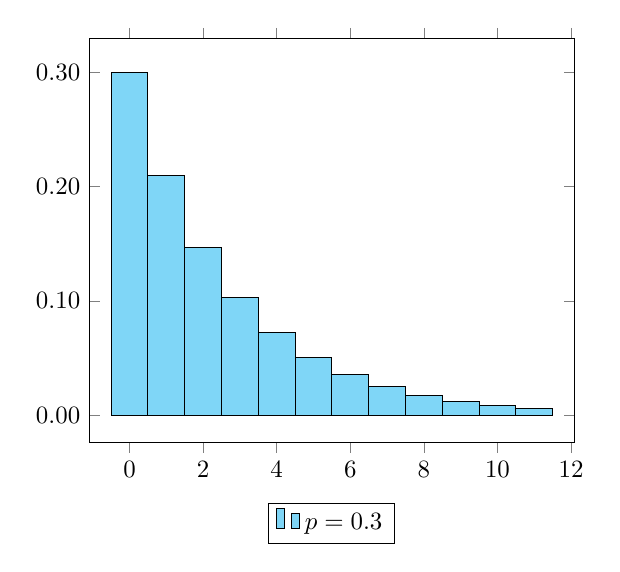
\begin{tikzpicture}[
        scale=0.9,
        declare function={geom(\k,\p)=(1-\p)^\k * \p;},
    ]
    \begin{axis}[
        samples at={0,...,11},
        yticklabel style={
            /pgf/number format/fixed,
            /pgf/number format/fixed zerofill,
            /pgf/number format/precision=2
        },
        legend style={at={(0.5, -0.15)},anchor=north},
        ybar=0pt, bar width=1
    ]
    \addplot [fill=cyan, fill opacity=0.5] {geom(x,0.3)}; \addlegendentry{$p=0.3$}
    \end{axis}
    \end{tikzpicture}
\end{minipage}
\begin{minipage}{0.49\textwidth}
    \centering
    \tikzsetnextfilename{424}
    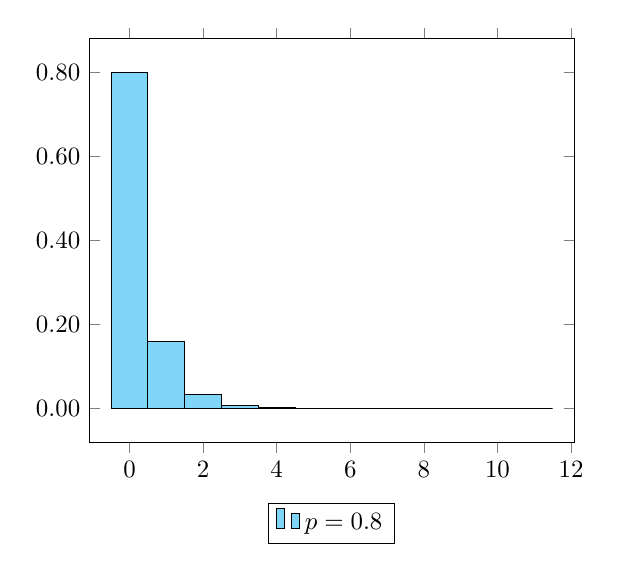
\begin{tikzpicture}[
        scale=0.9,
        declare function={geom(\k,\p)=(1-\p)^\k * \p;},
    ]
    \begin{axis}[
        samples at={0,...,11},
        yticklabel style={
            /pgf/number format/fixed,
            /pgf/number format/fixed zerofill,
            /pgf/number format/precision=2
        },
        legend style={at={(0.5, -0.15)},anchor=north},
        ybar=0pt, bar width=1
    ]
    \addplot [fill=cyan, fill opacity=0.5] {geom(x,0.8)}; \addlegendentry{$p=0.8$}
    \end{axis}
    \end{tikzpicture}
\end{minipage}

\medskip

All geometric distributions show this type of skewness (extreme positive skewness).